% Provenance (never printed): see sources/outline_sources.md (Year 1: continental
% rifting and break-up; passive-margin structure; fast and slow ridges; the depth--age
% law of the ocean floor; transform faults). Curve from figdata/bachelor-1/depth_age.py;
% exercise and problem values in the Book 3 scratch calculator calc/ch13.py; the
% coordinates of the margin schematic from calc/fig13_margin.py.
\chapter{Riftes, dorsais e margens passivas}\label{ch:b1:rifts-ridges-margins}

Em setembro de 2005 o solo do deserto de Afar, no nordeste da Etiópia, abriu-se. Em três semanas um trecho do rifte de cerca de \qty{60}{km} de comprimento alargou-se em até \qty{8}{m}, e cerca de \qty{2.5}{km^3} de magma subiu pela fenda vindo de baixo. As placas ali se separam a cerca de \qty{18}{mm} por ano: a crise liberou, em poucas semanas, o estiramento de uns quatro séculos. Afar é um continente se partindo; a algumas centenas de quilômetros ao norte, o mar Vermelho é um oceano jovem cujo fundo já é feito como o fundo do Atlântico, e o Atlântico Sul foi um rifte desse tipo antes de se abrir, cerca de 120 milhões de anos atrás. Este capítulo acompanha o nascimento de um oceano: o estiramento de um continente, sua fragmentação, as duas margens passivas deixadas para trás, a dorsal que constrói o fundo oceânico e o lento afundamento desse fundo à medida que esfria.
% ledger: wright:afar, morvel:ar-nb (18.5 mm/yr at 12.3 N, 40.6 E, computed with euler_velocities.py), heine:fit

\begin{recall}
As placas são a \omterm{def:b1:heat-budget:boundary-layer}{camada limite térmica} superior do \omterm{def:b1:layered-earth:layers}{manto}; sob os oceanos um semiespaço em resfriamento as descreve, e suas isotermas se aprofundam como a raiz quadrada da
idade (\cref{ch:b1:heat-budget}). Colunas de rocha em equilíbrio isostático têm a mesma massa por unidade de área acima de uma \omterm{def:b1:isostasy-gravity:isostasy}{profundidade de compensação}
(\cref{ch:b1:isostasy-gravity}). As placas giram em torno de \omterm{def:b1:plate-kinematics:euler-pole}{polos de Euler}, as dorsais se espalham a taxas lidas em anomalias magnéticas, e as transformantes estão sobre pequenos círculos em torno do polo (\cref{ch:b1:plate-kinematics}). O \omterm{def:b1:cross-sections:throw}{rejeito} e o \omterm{def:b1:cross-sections:throw}{afastamento horizontal} de uma falha foram definidos em \cref{ch:b1:cross-sections}; uma falha normal é uma falha inclinada cujo bloco superior desceu (Livro 2, 11º ano).
\end{recall}

\section{Rifteamento continental}

Um continente esticado por forças em suas bordas não se afina de modo uniforme. Sua \omterm{def:b1:layered-earth:layers}{crosta} superior frágil se quebra ao longo de falhas normais, e os blocos entre elas afundam e
inclinam-se; embaixo, a \omterm{def:b1:layered-earth:layers}{crosta} inferior mais quente e o \omterm{def:b1:layered-earth:layers}{manto} escoam.

\begin{definition}[Rifte continental, gráben, semigráben]\label{def:b1:rifts-ridges-margins:rift}
Um \emph{rifte continental}\index{rifte continental} é uma zona longa e estreita onde um continente está sendo esticado: uma depressão limitada por falhas normais, com terremotos e, com frequência, vulcões. Um \emph{gráben}\index{gráben} é um bloco abatido entre duas falhas normais que mergulham uma na direção da outra. Um
\emph{semigráben}\index{semigráben} é um bloco abatido e inclinado contra uma única falha normal principal, a falha de borda, em apenas um dos lados.
\end{definition}

A maioria das bacias de rifte é uma cadeia de \omterm{def:b1:rifts-ridges-margins:rift}{semigrábens}. Suas falhas de borda transferem o deslocamento umas às outras por rampas de revezamento, e o lado em que
fica a falha de borda muitas vezes se alterna de um segmento para o seguinte. O bloco de teto de cada falha de borda inclina-se para baixo em direção a ela, e a bacia se enche mais depressa ali:
o sedimento mais espesso se acumula contra a falha, enquanto o bloco de base é erguido na ombreira do rifte.

O estiramento horizontal transportado por uma falha é o seu \omterm{def:b1:cross-sections:throw}{afastamento horizontal}. Uma falha normal planar de \omterm{def:b1:cross-sections:throw}{rejeito} $h$ e \omterm{def:b1:geological-maps:attitude}{mergulho} $\delta$ tem \omterm{def:b1:cross-sections:throw}{afastamento horizontal} $h/\tan\delta$
(\cref{ch:b1:cross-sections}); somando os afastamentos horizontais das falhas através de uma seção de rifte obtém-se a extensão da \omterm{def:b1:layered-earth:layers}{crosta} frágil. Como toda a \omterm{def:b1:layered-earth:lithosphere}{litosfera} se afina ao ser esticada, e por que depois ela afunda, é quantificado no Livro 4; aqui as falhas são medidas, e sua soma comparada com o movimento das placas.

\begin{omfigure}
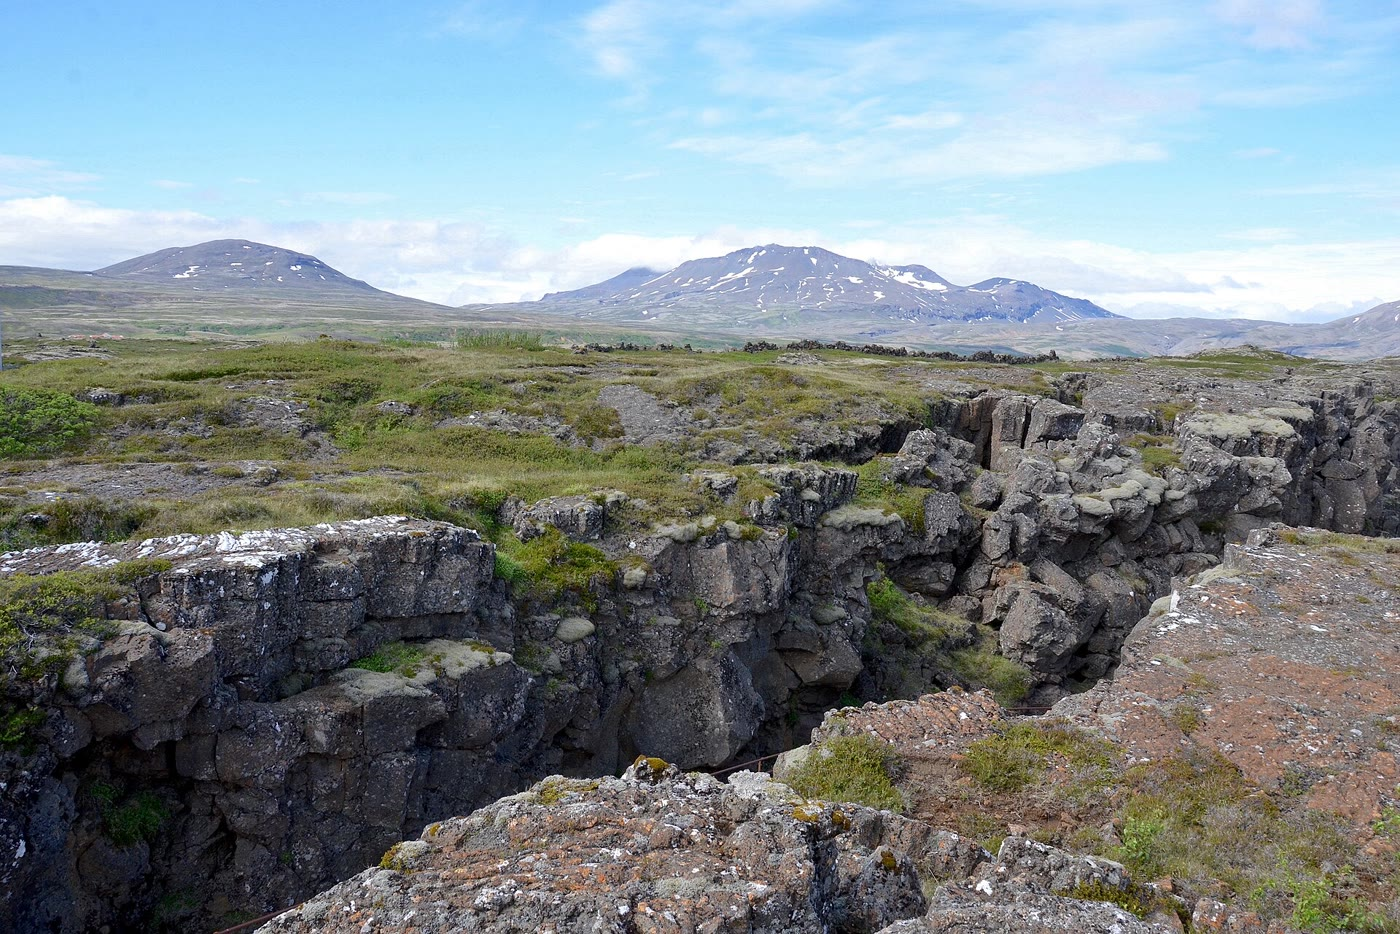
\includegraphics[width=0.8\linewidth]{images/book3/b1-thingvellir-fissure.jpg}

\par\smallskip{\small Uma fenda aberta no piso de lava do vale de rifte de Þingvellir,
no sudoeste da Islândia, onde a Dorsal Meso-Atlântica aflora. Os fluxos de basalto do fundo do vale são cortados por fendas abertas paralelas ao rifte. Fotografia: Olga Ernst,
CC~BY-SA~4.0 (Wikimedia Commons).}
\label{fig:b1:rifts-ridges-margins:thingvellir}
\end{omfigure}
% ledger: commons:thingvellir

\subsection*{Riftes vulcânicos e pobres em magma}

Riftes diferem na quantidade de magma que recebem. Em um rifte \emph{pobre em magma} o estiramento é absorvido por falhas, e a \omterm{def:b1:layered-earth:layers}{crosta} se afina à medida que os blocos deslizam
afastados. Em um rifte vulcânico o magma toma o lugar: diques intrudem a \omterm{def:b1:layered-earth:layers}{crosta} ao longo do eixo, cada um abrindo o rifte por sua própria espessura, e lavas inundam a superfície. O Rifte da África Oriental mostra os dois, lado a lado: seu ramo leste
é fortemente vulcânico, enquanto seu ramo oeste é menos, e abriga bacias sedimentares profundas, preenchidas por lagos como o Tanganica e limitadas por falhas.
% ledger: roberts:ear

Os dois ramos começaram a se formar cerca de 25 milhões de anos atrás, e o rifte divide a placa africana em uma placa núbia, a oeste, e uma placa somali, a leste. A partir da \omterm{def:b1:plate-kinematics:triple-junction}{junção tripla} de Afar ele segue para o sul, em dois ramos em torno do antigo, espesso e frio cráton da Tanzânia.
Seu movimento é lento: calculado a partir dos vetores de placa da Somália e da Núbia, cada um medido em relação à placa antártica, a Somália se afasta da Núbia a \qty{6.0}{mm.yr^{-1}} em direção a \ang{105} no centro da Etiópia (\ang{8.5}\,N, \ang{39.5}\,L), e a \qty{5.1}{mm.yr^{-1}} na linha do equador.
Muitos terremotos do rifte mostram falhamento normal.
% ledger: roberts:ear, morvel:sm-an, morvel:nb-an (SM-NB from SM-AN minus NB-AN, computed with figdata/bachelor-1/euler_velocities.py)

Em Afar, na extremidade norte, o rifte encontra o mar Vermelho e o golfo de Áden. A maior parte dos basaltos de inundação da Etiópia entrou ali cerca de 30 milhões de anos atrás, em um milhão de anos ou menos, e o magma continuou a chegar desde então: lavas escorrem na superfície, intrusões ocorrem na \omterm{def:b1:layered-earth:layers}{crosta} e material novo é acrescentado abaixo dela, tanto que a \omterm{def:b1:layered-earth:layers}{crosta} intrudida manteve sua espessura durante as primeiras fases do rifteamento.
A crise de 2005 mostra como um rifte desse tipo se abre: não de modo constante, mas em episódios, cada um um dique de metros de largura intrudido em dias ou semanas. Como as placas divergem a cerca de \qty{18}{mm.yr^{-1}} ali, o dique de \qty{8}{m} de 2005 absorveu o estiramento de cerca de 440 anos.
% ledger: hofmann:traps, bastow:afar, wright:afar, morvel:ar-nb (rate computed with euler_velocities.py)

\section{Ruptura e margens passivas}

Se o estiramento continua, a \omterm{def:b1:layered-earth:layers}{crosta} continental se afina até desaparecer, o \omterm{def:b1:layered-earth:layers}{manto} sobe sob o rifte e se funde à medida que sobe, e a primeira \omterm{def:b1:rifts-ridges-margins:oceanic-crust}{crosta oceânica} se forma entre as duas metades do continente. Esse momento é a \emph{ruptura}. A partir daí as placas se afastam em uma dorsal no meio de um oceano novo, e as duas bordas do continente, levadas para longe da dorsal, deixam de ser fronteiras de placas.

\begin{definition}[Margem passiva, transição oceano--continente, discordância de ruptura]\label{def:b1:rifts-ridges-margins:passive-margin}
Uma \emph{margem passiva}\index{margem passiva} é a borda de um continente formada por rifteamento e que não é mais uma fronteira de placas: o continente e o fundo oceânico adjacente pertencem à mesma placa. A
\emph{transição oceano--continente}\index{transição oceano--continente} é a zona da margem, de quilômetros a dezenas de quilômetros de largura, entre a \omterm{def:b1:layered-earth:layers}{crosta} continental afinada e a \omterm{def:b1:rifts-ridges-margins:oceanic-crust}{crosta oceânica} normal. A \emph{discordância de ruptura}\index{discordância de ruptura} é a \omterm{def:b1:cross-sections:unconformity}{discordância} que separa
os sedimentos depositados nas bacias de rifte, inclinados junto com seus blocos, dos sedimentos não perturbados depositados sobre a margem depois da ruptura.
\end{definition}

Margens passivas bordejam a maior parte do Atlântico, o oceano Ártico e a parte oeste do oceano Índico, e quase todas as costas da África, da Austrália, da Groenlândia e da Índia. A margem leste da América do Norte e a margem noroeste da África foram os dois lados de um único rifte: são margens \emph{conjugadas}. Seu perfil é a sequência familiar do fundo oceânico junto à terra: plataforma continental, talude, sopé continental e planície abissal. Sob a plataforma e o talude jaz a \omterm{def:b1:layered-earth:layers}{crosta} continental afinada, cortada por falhas normais que mergulham para o oceano, com seus blocos rotacionados enterrados sob os sedimentos.

\begin{omfigure}
\begin{tikzpicture}[x=0.95cm, y=0.9cm, font=\scriptsize]
% (a) continental rift: half-grabens on east-dipping faults; coordinates from calc/fig13_margin.py
\begin{scope}
\fill[green!25!gray!45] (0,-2) -- (3,-2) -- (6,-1.75) -- (9,-2) -- (12,-2) -- (12,-2.5) -- (0,-2.5) -- cycle;
\fill[orange!22] (0,0) -- (3.5,0) -- (3.931,-0.8) -- (4.75,-0.25) -- (5.05,-0.7) -- (6,-0.2) -- (6.223,-0.55) -- (7.25,-0.15) -- (7.402,-0.4) -- (8.6,0) -- (12,0) -- (12,-2) -- (9,-2) -- (6,-1.75) -- (3,-2) -- (0,-2) -- cycle;
\fill[yellow!45] (3.565,-0.12) -- (3.931,-0.8) -- (4.75,-0.25) -- (4.75,-0.12) -- cycle;
\fill[yellow!45] (4.75,-0.12) -- (4.75,-0.25) -- (5.05,-0.7) -- (6,-0.2) -- (6,-0.12) -- cycle;
\fill[yellow!45] (6,-0.12) -- (6,-0.2) -- (6.223,-0.55) -- (7.25,-0.15) -- (7.25,-0.12) -- cycle;
\fill[yellow!45] (7.25,-0.12) -- (7.25,-0.15) -- (7.402,-0.4) -- (8.241,-0.12) -- cycle;
\draw (0,0) -- (3.5,0) -- (3.931,-0.8) -- (4.75,-0.25) -- (5.05,-0.7) -- (6,-0.2) -- (6.223,-0.55) -- (7.25,-0.15) -- (7.402,-0.4) -- (8.6,0) -- (12,0);
\draw[contact] (0,-2) -- (3,-2) -- (6,-1.75) -- (9,-2) -- (12,-2);
\draw[fault] (3.5,0) -- (4.2,-1.3);
\draw[fault] (4.75,-0.25) -- (5.45,-1.3);
\draw[fault] (6,-0.2) -- (6.7,-1.3);
\draw[fault] (7.25,-0.15) -- (7.95,-1.3);
\node[anchor=west, font=\small\bfseries] at (0,0.75) {(a) rifte continental};
\node[anchor=south] at (2.2,0) {ombreira do rifte};
\node[anchor=south, align=center] at (6.3,0) {semigrábens preenchidos com sedimento};
\draw[-{Stealth[length=3pt]}] (2.6,-0.75) node[anchor=east] {falha de borda} -- (3.75,-0.5);
\node at (9.8,-1.0) {crosta continental};
\node at (10.3,-2.25) {manto};
\node at (6,-2.18) {Moho elevado sob o rifte};
\end{scope}
% (b) break-up: conjugate halves, the first oceanic crust between them
\begin{scope}[yshift=-3.6cm]
\fill[omSea!35] (2.8,0) -- (9.2,0) -- (9.2,-1.3) -- (2.8,-1.3) -- cycle;
\fill[green!25!gray!45] (0,-2) -- (2.5,-2) -- (5.5,-1.3) -- (6.5,-1.3) -- (9.5,-2) -- (12,-2) -- (12,-2.5) -- (0,-2.5) -- cycle;
\fill[orange!22] (0,0) -- (2.8,0) -- (3.146,-0.75) -- (3.8,-0.3) -- (4.13,-0.85) -- (4.7,-0.45) -- (5.053,-0.95) -- (5.5,-1) -- (5.5,-1.3) -- (2.5,-2) -- (0,-2) -- cycle;
\fill[orange!22] (12,0) -- (9.2,0) -- (8.854,-0.75) -- (8.2,-0.3) -- (7.87,-0.85) -- (7.3,-0.45) -- (6.947,-0.95) -- (6.5,-1) -- (6.5,-1.3) -- (9.5,-2) -- (12,-2) -- cycle;
\fill[lith basalt] (5.5,-1) -- (6.5,-1) -- (6.5,-1.3) -- (5.5,-1.3) -- cycle;
\draw (0,0) -- (2.8,0) -- (3.146,-0.75) -- (3.8,-0.3) -- (4.13,-0.85) -- (4.7,-0.45) -- (5.053,-0.95) -- (5.5,-1) -- (6.5,-1) -- (6.947,-0.95) -- (7.3,-0.45) -- (7.87,-0.85) -- (8.2,-0.3) -- (8.854,-0.75) -- (9.2,0) -- (12,0);
\draw[contact] (0,-2) -- (2.5,-2) -- (5.5,-1.3) -- (6.5,-1.3) -- (9.5,-2) -- (12,-2);
\draw[omSea!70!black] (2.8,0) -- (9.2,0);
\draw[fault] (2.8,0) -- (3.4,-1.3);
\draw[fault] (3.8,-0.3) -- (4.4,-1.3);
\draw[fault] (4.7,-0.45) -- (5.3,-1.3);
\draw[fault] (9.2,0) -- (8.6,-1.3);
\draw[fault] (8.2,-0.3) -- (7.6,-1.3);
\draw[fault] (7.3,-0.45) -- (6.7,-1.3);
\draw[omRidge, very thick, -{Stealth[length=3pt]}] (6,-2.3) -- (6,-1.45);
\node[anchor=west, font=\small\bfseries] at (0,0.75) {(b) ruptura};
\node[anchor=south] at (6,0) {o mar inunda o rifte};
\node[anchor=west] at (6.15,-2.1) {o manto sobe e se funde};
\node[anchor=south, fill=white, fill opacity=0.8, text opacity=1, inner sep=1pt, align=center] at (6,-0.85) {primeira\\crosta oceânica};
\node at (1.4,-1.0) {blocos inclinados};
\node at (10.6,-1.0) {blocos inclinados};
\node at (1.4,-2.25) {manto};
\end{scope}
% (c) one passive margin after drift
\begin{scope}[yshift=-7.4cm]
\fill[omSea!35] (1.2,0.3) -- (12,0.3) -- (12,-1.2) -- (8.2,-1.15) -- (6.4,-0.9) -- (4.6,0.1) -- cycle;
\fill[green!25!gray!45] (0,-2.3) -- (2,-2.3) -- (5.9,-1.8) -- (6.7,-2.1) -- (12,-2.1) -- (12,-2.7) -- (0,-2.7) -- cycle;
\fill[orange!22] (0,0.3) -- (1.2,0.3) -- (2.2,0) -- (3,-0.25) -- (3.259,-0.95) -- (4,-0.55) -- (4.286,-1.15) -- (4.9,-0.85) -- (5.233,-1.35) -- (5.9,-1.55) -- (5.9,-1.8) -- (2,-2.3) -- (0,-2.3) -- cycle;
\fill[pattern=crosshatch dots, pattern color=green!40!black] (5.9,-1.55) -- (6.4,-1.75) -- (6.7,-2.1) -- (5.9,-1.8) -- cycle;
\fill[lith basalt] (6.4,-1.75) -- (12,-1.75) -- (12,-2.1) -- (6.7,-2.1) -- cycle;
\fill[yellow!45] (3,-0.25) -- (3.259,-0.95) -- (4,-0.55) -- cycle;
\fill[yellow!45] (4,-0.55) -- (4.286,-1.15) -- (4.9,-0.85) -- cycle;
\fill[yellow!45] (4.9,-0.85) -- (5.233,-1.35) -- (5.9,-1.55) -- (5.9,-1.45) -- cycle;
\fill[yellow!15] (1.2,0.3) -- (4.6,0.1) -- (6.4,-0.9) -- (8.2,-1.15) -- (12,-1.2) -- (12,-1.75) -- (6.4,-1.75) -- (5.9,-1.55) -- (5.9,-1.45) -- (4.9,-0.85) -- (4,-0.55) -- (3,-0.25) -- (2.2,0) -- cycle;
\draw[black!45] (2.4,0.12) -- (4.8,-0.1) -- (6.6,-1.05) -- (8.4,-1.27) -- (12,-1.31);
\draw (1.2,0.3) -- (4.6,0.1) -- (6.4,-0.9) -- (8.2,-1.15) -- (12,-1.2);
\draw[omSea!70!black] (1.2,0.3) -- (12,0.3);
\draw[unconformity] (2.2,0) -- (3,-0.25) -- (4,-0.55) -- (4.9,-0.85) -- (5.9,-1.45);
\draw (3.259,-0.95) -- (4,-0.55) (4.286,-1.15) -- (4.9,-0.85) (5.233,-1.35) -- (5.9,-1.55) -- (6.4,-1.75) -- (12,-1.75);
\draw[contact] (0,-2.3) -- (2,-2.3) -- (5.9,-1.8) -- (6.7,-2.1) -- (12,-2.1);
\draw[fault] (3,-0.25) -- (3.5,-1.6);
\draw[fault] (4,-0.55) -- (4.5,-1.6);
\draw[fault] (4.9,-0.85) -- (5.4,-1.6);
\node[anchor=west, font=\small\bfseries] at (0,0.95) {(c) margem passiva};
\node[anchor=south] at (3.4,0.25) {plataforma};
\node[anchor=south west] at (5.6,-0.45) {talude};
\node[anchor=south] at (8.4,-1.12) {sopé};
\node[anchor=south] at (10.6,-1.17) {planície abissal};
\node[anchor=south] at (10.6,-0.1) {oceano};
\node at (9.8,-1.53) {sedimentos pós-rifte};
\node[fill=white, fill opacity=0.8, text opacity=1, inner sep=1pt, align=center] (bu) at (1.0,-0.6) {discordância\\de ruptura};
\draw[-{Stealth[length=3pt]}] (bu.east) -- (2.55,-0.16);
\node[fill=white, fill opacity=0.8, text opacity=1, inner sep=1pt, align=center] (sr) at (1.6,-1.35) {sedimentos\\sinrifte};
\draw[-{Stealth[length=3pt]}] (sr.east) -- (3.45,-0.75);
\node at (1.3,-1.98) {crosta continental};
\draw[decorate, decoration={brace, amplitude=3pt, mirror}] (5.9,-2.17) -- (6.7,-2.17) node[midway, below=3pt, align=center] {transição\\oceano--continente};
\node[anchor=west, fill=white, fill opacity=0.85, text opacity=1, inner sep=1pt] at (8.6,-1.93) {crosta oceânica};
\node at (3.6,-2.5) {manto};
\end{scope}
\end{tikzpicture}

\par\smallskip{\small Do rifte à \omterm{def:b1:rifts-ridges-margins:passive-margin}{margem passiva} (desenhos, fora de escala; as alturas são exageradas). (a) A \omterm{def:b1:layered-earth:layers}{crosta} superior frágil se quebra ao longo de falhas normais; blocos inclinam-se em \omterm{def:b1:rifts-ridges-margins:rift}{semigrábens} que se enchem de sedimento, e o \omterm{def:b1:layered-earth:discontinuity}{Moho} sobe sob a \omterm{def:b1:layered-earth:layers}{crosta} afinada. (b) Na ruptura a \omterm{def:b1:layered-earth:layers}{crosta} continental é cortada até o fim; o mar inunda o rifte e forma-se a primeira \omterm{def:b1:rifts-ridges-margins:oceanic-crust}{crosta oceânica}. (c) Uma das duas margens, levada para longe da dorsal: seus blocos inclinados e seus sedimentos jazem sob a \omterm{def:b1:rifts-ridges-margins:passive-margin}{discordância de ruptura}, enterrados pelos sedimentos pós-rifte da plataforma, do talude e do sopé.}
\label{fig:b1:rifts-ridges-margins:margin}
\end{omfigure}

\subsection*{Dois tipos de margem}

As margens herdam o caráter de seu rifte. Em margens \emph{pobres em magma}, como as da Ibéria e de Terra Nova, as seções sísmicas mostram blocos rotacionados cujas camadas mergulham para o continente; em alguns lugares a \omterm{def:b1:rifts-ridges-margins:passive-margin}{transição oceano--continente} é assentada por peridotito do \omterm{def:b1:layered-earth:layers}{manto}, trazido ao fundo do mar e alterado pela água do mar a serpentinito.
Em margens \emph{vulcânicas}, como as margens do centro da Noruega, da Groenlândia oriental, da Namíbia e do Brasil, a transição é construída de basalto: pilhas de fluxos de lava que mergulham para o oceano, os refletores que mergulham para o mar das seções sísmicas, e abaixo deles uma \omterm{def:b1:layered-earth:layers}{crosta} inferior na qual ondas P viajam anormalmente depressa, com magma acrescentado sob a \omterm{def:b1:layered-earth:layers}{crosta} na ruptura. Margens vulcânicas afundam pouco durante a ruptura.

\begin{inthefield}[Encontrar a borda de um continente]
A \omterm{def:b1:rifts-ridges-margins:passive-margin}{transição oceano--continente} fica sob quilômetros de água e sedimento, e só é localizada pela geofísica, em geral por vários métodos juntos.
A reflexão sísmica gera imagens dos blocos inclinados, da \omterm{def:b1:rifts-ridges-margins:passive-margin}{discordância de ruptura} e, quando o sinal chega fundo o bastante, do \omterm{def:b1:layered-earth:discontinuity}{Moho}. A refração sísmica de grande ângulo mede as velocidades das ondas P através da \omterm{def:b1:layered-earth:layers}{crosta}, que diferem entre \omterm{def:b1:layered-earth:layers}{crosta} continental e oceânica.
Os dados gravimétricos, invertidos para a profundidade do \omterm{def:b1:layered-earth:discontinuity}{Moho}, dão a espessura da \omterm{def:b1:layered-earth:layers}{crosta}. As listras magnéticas do fundo oceânico param onde começa a \omterm{def:b1:layered-earth:layers}{crosta} continental, magneticamente silenciosa.
\end{inthefield}

Depois da ruptura, uma margem afunda. Durante o rifteamento a \omterm{def:b1:layered-earth:lithosphere}{litosfera} foi afinada e aquecida; levada para longe da dorsal, ela esfria e se contrai, como o fundo oceânico ao lado, e o espaço que se abre sobre ela se enche com a cunha de sedimentos pós-rifte, cujo peso a empurra ainda mais para baixo.
A metade de resfriamento dessa história é contada em \cref{sec:b1:rifts-ridges-margins:depth-age}; o peso dos sedimentos é o tema de \cref{ch:b1:diagenesis-basins}.

\section{Dorsais rápidas e lentas}

Uma vez nascido, o oceano cresce em sua dorsal. As dorsais se espalham a taxas muito diferentes: as taxas medidas nos últimos milhões de anos vão de \qty{9.7}{mm.yr^{-1}} no norte do mar Vermelho a \qty{154.4}{mm.yr^{-1}} na Dorsal do Pacífico Leste. A forma delas depende dessa taxa.
% ledger: morvel:range

\begin{definition}[Dorsais de espalhamento rápido, lento e ultralento]\label{def:b1:rifts-ridges-margins:ridge-classes}
Uma dorsal é classificada pela sua \omterm{def:b1:plate-kinematics:spreading-rate}{taxa de espalhamento completa}. Uma
\emph{dorsal de espalhamento ultralento}\index{dorsal de espalhamento ultralento} abre-se a menos de cerca de \qty{20}{mm.yr^{-1}}; uma \emph{dorsal de espalhamento lento}\index{dorsal de espalhamento lento} a 20 a \qty{55}{mm.yr^{-1}}; uma dorsal intermediária a 55 a \qty{75}{mm.yr^{-1}}; uma \emph{dorsal de espalhamento rápido}\index{dorsal de espalhamento rápido} a mais de cerca de \qty{75}{mm.yr^{-1}}.
\end{definition}
% ledger: seton:rate-classes, dick:ultraslow

Os limites são convenções e variam entre autores. O que não varia é a mudança de forma. Uma dorsal lenta, como a Dorsal Meso-Atlântica, tem um vale axial entre falhas normais voltadas para dentro: a fenda entre as placas não é preenchida por magma tão depressa quanto se abre, e a \omterm{def:b1:layered-earth:lithosphere}{litosfera} fria se quebra. Uma dorsal rápida, como a Dorsal do Pacífico Leste, não tem vale de rifte, mas um alto axial liso sobre uma lente de fusão, reabastecida com frequência suficiente para acompanhar.
De qualquer modo o eixo fica a cerca de \qty{2500}{m} de profundidade, e o fundo mais antigo das bacias quase \qty{4}{km} mais fundo (\cref{sec:b1:rifts-ridges-margins:depth-age}).
% ledger: parsons:plate-model (6400 - 2500 m)

Dorsais ultralentas mostram o que acontece quando o magma é mais escasso: seu vulcanismo é intermitente, elas não têm transformantes e, em grandes regiões, o próprio \omterm{def:b1:layered-earth:layers}{manto} é trazido ao fundo do mar. A Dorsal de Gakkel, sob o oceano Ártico, a mais lenta de todas, não tem nenhum deslocamento; ao longo de um trecho central de seu eixo com cerca de \qty{300}{km} de comprimento, peridotito do \omterm{def:b1:layered-earth:layers}{manto} jaz diretamente sobre o eixo, entre um vulcanismo abundante a oeste e grandes vulcões espaçados a leste.
Em dorsais lentas e ultralentas, especialmente, parte do espalhamento é absorvida por falhas normais longas e pouco inclinadas, descolamentos, cujo bloco de base é puxado para fora de sob o eixo: gabro e peridotito chegam ao fundo do mar em domos corrugados, \emph{complexos de núcleo oceânicos}. O Atlantis Massif, ao lado da Dorsal Meso-Atlântica perto de \ang{30}\,N, é um deles: em seu topo, sobre \omterm{def:b1:layered-earth:layers}{crosta} de \qty{1.5}{Myr} a cerca de \qty{15}{km} do eixo, a água do mar reagindo com a rocha do \omterm{def:b1:layered-earth:layers}{manto} alimenta as fontes quentes e alcalinas do campo hidrotermal Lost City.
% ledger: dick:ultraslow, michael:gakkel, kelley:lost-city

\subsection*{A crosta oceânica}

\begin{definition}[Crosta oceânica, lava em almofada, complexo de diques em lençol]\label{def:b1:rifts-ridges-margins:oceanic-crust}
A \emph{crosta oceânica}\index{crosta oceânica} é a \omterm{def:b1:layered-earth:layers}{crosta} formada nas dorsais oceânicas: de 6 a \qty{7}{km} de basalto e gabro, do fundo do mar até o \omterm{def:b1:layered-earth:discontinuity}{Moho}, sob uma cobertura de sedimentos.
A \emph{lava em almofada}\index{lava em almofada} é lava erupcionada sob a água, feita de tubos e lóbulos arredondados e interligados, cada um com uma pele vítrea resfriada pelo mar. Um \emph{complexo de diques em lençol}\index{complexo de diques em lençol} é uma camada feita quase inteiramente de diques verticais paralelos, cada um intrudido entre os anteriores.
\end{definition}

As camadas da \omterm{def:b1:rifts-ridges-margins:oceanic-crust}{crosta oceânica} foram definidas primeiro pela sismologia, depois amostradas por perfuração e reconhecidas em fatias de fundo oceânico empurradas sobre os continentes, os ofiolitos. Do topo:
\begin{itemize}
  \item camada~1, sedimentos, finos ou ausentes perto da dorsal e engrossando com
        a idade do fundo;
  \item camada~2, em média \qty{1.84}{km} de basalto: \omterm{def:b1:rifts-ridges-margins:oceanic-crust}{lava em almofada} no topo
        (camada~2A), diques em lençol de diabásio embaixo (camada~2B);
  \item camada~3, os quatro a cinco quilômetros restantes, de gabro e, em sua base, cumulados depositados a partir do magma: cerca de \qty{70}{\percent} da
        espessura da \omterm{def:b1:layered-earth:layers}{crosta}.
\end{itemize}
Abaixo do \omterm{def:b1:layered-earth:discontinuity}{Moho} jaz peridotito do \omterm{def:b1:layered-earth:layers}{manto}, o resíduo deixado pela fusão.
% ledger: christeson:crust, white:crust (layer 3: 6.15 - 1.84 = 4.3 km, 70 %; 7.1 - 1.84 = 5.3 km)

A refração sísmica dá à \omterm{def:b1:layered-earth:layers}{crosta} ígnea uma espessura média de
\qty[uncertainty-mode=separate]{7.1 \pm 0.8}{km} longe das \omterm{def:b1:rifts-ridges-margins:transform}{zonas de fratura} e dos pontos quentes, e uma síntese posterior de perfis sísmicos dá \qty{6.15}{km}, quase a mesma em todas as taxas de espalhamento: a quantidade de fusão depende da temperatura do \omterm{def:b1:layered-earth:layers}{manto} ascendente, não da velocidade com que ele sobe. Apenas dorsais muito lentas produzem \omterm{def:b1:layered-earth:layers}{crosta} anormalmente fina: o \omterm{def:b1:layered-earth:layers}{manto} ali tem tempo de esfriar enquanto sobe, e funde menos. Sobre uma pluma quente a \omterm{def:b1:layered-earth:layers}{crosta} é mais espessa, cerca de \qty{20}{km} diretamente acima do núcleo ascendente de uma pluma, como sob a Islândia (\cref{ch:b1:hotspots}). Ao longo de todas as dorsais juntas, cerca de \qty{3.0}{km^2} de novo fundo oceânico e cerca de \qty{20}{km^3} de nova \omterm{def:b1:layered-earth:layers}{crosta} são produzidos a cada ano.
% ledger: white:crust, christeson:crust, data:pb2002 (production summed over the spreading steps in figdata/bachelor-1/ridge_budget.py)

\begin{omfigure}
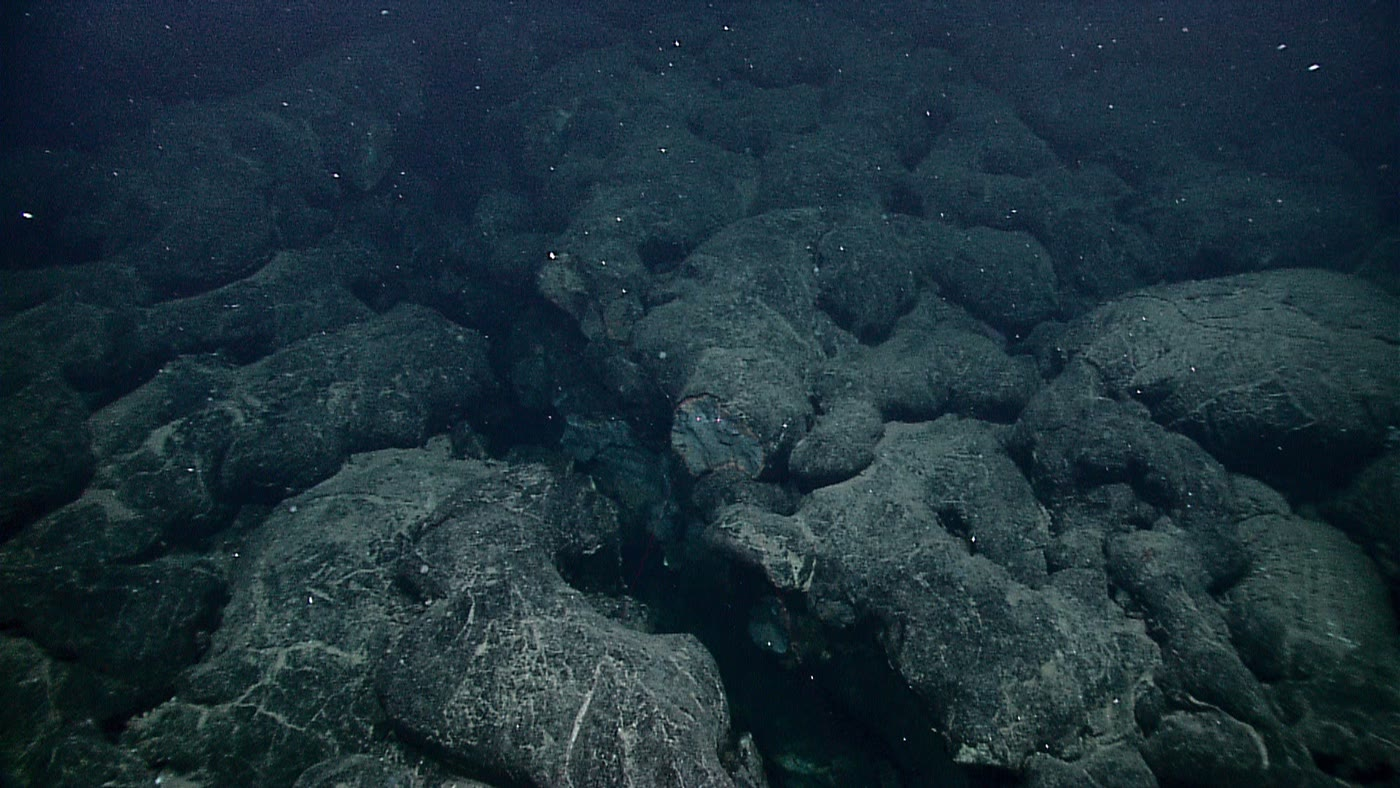
\includegraphics[width=0.6\linewidth]{images/book3/b1-pillow-lava.jpg}

\par\smallskip{\small \omterm{def:b1:rifts-ridges-margins:oceanic-crust}{Lavas em almofada} no Rifte de Galápagos, cortadas por uma fenda
que se abriu depois que elas tinham endurecido: o topo da camada~2 da \omterm{def:b1:rifts-ridges-margins:oceanic-crust}{crosta oceânica} no momento em que se forma. Cada almofada é uma língua de lava congelada por fora pela água do mar. Fotografia: NOAA Okeanos Explorer Program, Galápagos Rift Expedition
2011, CC~BY~2.0 (Wikimedia Commons).}
\label{fig:b1:rifts-ridges-margins:pillows}
\end{omfigure}
% ledger: commons:pillow-expl6453

\begin{proposition}[Cada dique divide o anterior]\label{prop:b1:rifts-ridges-margins:dykes}
Suponha que cada dique de um \omterm{def:b1:rifts-ridges-margins:oceanic-crust}{complexo de diques em lençol} seja intrudido ao longo do eixo de espalhamento, onde a \omterm{def:b1:layered-earth:layers}{crosta} é mais quente e mais fraca, e que a \omterm{def:b1:layered-earth:layers}{crosta} se afaste do eixo simetricamente. Então a maioria dos diques é encontrada partida em duas, cada
metade com uma margem resfriada apenas contra seu vizinho mais antigo.
\end{proposition}

\begin{proof}
Um dique esfria contra a rocha mais fria dos dois lados: ele tem duas margens resfriadas quando se forma. O dique seguinte sobe onde a \omterm{def:b1:layered-earth:layers}{crosta} é mais fraca, ao longo do eixo, isto é, pelo meio do anterior, ainda a rocha mais quente.
Ele o divide em duas metades, que o espalhamento leva para os dois lados; cada metade mantém a margem resfriada de seu lado externo e tem, em seu lado interno, o contato não resfriado com o novo dique. Todo dique, exceto o último, é dividido desse modo.
\end{proof}

Diques com margem resfriada de um lado só são, de fato, a regra nos \omterm{def:b1:rifts-ridges-margins:oceanic-crust}{complexos de diques em lençol}: a assinatura de uma \omterm{def:b1:layered-earth:layers}{crosta} construída, dique após dique, pelo espalhamento.


\section{A lei profundidade--idade}\label{sec:b1:rifts-ridges-margins:depth-age}

O fundo oceânico é raso na dorsal e fundo longe dela. Como o fundo se forma na dorsal e é levado para longe, a distância da dorsal é a idade, e a profundidade do fundo depende de sua idade. A placa esfria por cima à medida que envelhece (\cref{ch:b1:heat-budget}); rocha fria é mais densa, e uma coluna mais densa flutua mais baixo.

\begin{lemma}[Uma integral da função erro]\label{lem:b1:rifts-ridges-margins:erfc}
Com $\operatorname{erfc} u = 1 - \operatorname{erf} u =
\frac{2}{\sqrt\pi}\int_u^\infty e^{-s^2}\,\mathrm ds$,
\[
  \int_0^\infty \operatorname{erfc} u \,\mathrm du = \frac{1}{\sqrt\pi}.
\]
\end{lemma}

\begin{proof}
A derivada de $\operatorname{erfc}$ é $-\frac{2}{\sqrt\pi}e^{-u^2}$.
Integrando por partes em $[0, X]$,
\[
  \int_0^X \operatorname{erfc} u\,\mathrm du
  = \bigl[u \operatorname{erfc} u\bigr]_0^X + \frac{2}{\sqrt\pi}\int_0^X u\,e^{-u^2}\,\mathrm du
  = X\operatorname{erfc} X + \frac{1}{\sqrt\pi}\bigl(1 - e^{-X^2}\bigr).
\]
Para $X > 0$ e $s \ge X$, $e^{-s^2} \le (s/X)e^{-s^2}$, logo
$X\operatorname{erfc} X \le \frac{2}{\sqrt\pi}\int_X^\infty s\,e^{-s^2}\,\mathrm ds
= e^{-X^2}/\sqrt\pi$, que tende a 0. Fazendo $X \to \infty$ obtém-se o
resultado.
\end{proof}

\begin{theorem}[Lei profundidade--idade]\label{thm:b1:rifts-ridges-margins:depth-age}
Suponha que
\begin{enumerate}
  \item o \omterm{def:b1:layered-earth:layers}{manto} deixa a dorsal à temperatura uniforme $T_m$, e a placa oceânica de idade $t$ é um semiespaço resfriado desde então a partir de sua superfície, mantida em $T_0$, com a difusividade térmica $\kappa$;
  \item a densidade da rocha resfriada é $\rho_m\bigl(1 + \alpha(T_m -
        T)\bigr)$, com $\rho_m$ a densidade do \omterm{def:b1:layered-earth:layers}{manto} em $T_m$ e
        $\alpha$ seu coeficiente de expansão térmica;
  \item cada coluna está em equilíbrio isostático acima de uma \omterm{def:b1:isostasy-gravity:isostasy}{profundidade de compensação}
        situada abaixo da camada resfriada, e a água do mar tem densidade $\rho_w$.
\end{enumerate}
Então a profundidade do fundo do mar de idade $t$ é
\[
  d(t) = d_r + C\sqrt t, \qquad
  C = \frac{2}{\sqrt\pi}\,\frac{\rho_m\,\alpha\,(T_m - T_0)\sqrt\kappa}{\rho_m - \rho_w},
\]
onde $d_r$ é a profundidade do eixo da dorsal. Esta é a
\emph{lei profundidade--idade}\index{lei profundidade--idade} do fundo oceânico.
\end{theorem}

\begin{proof}
A temperatura no semiespaço resfriado é
\[
  T(z, t) = T_0 + (T_m - T_0)\operatorname{erf}\frac{z}{2\sqrt{\kappa t}},
\]
com $z$ a profundidade abaixo do fundo do mar; esta solução da equação do calor é
admitida aqui, como em \cref{ch:b1:heat-budget}, e deduzida no Livro 5. Compare a coluna na dorsal, feita de água até $d_r$ e de
\omterm{def:b1:layered-earth:layers}{manto} a $T_m$ embaixo, com a coluna de idade $t$, feita de água até $d$ e
da placa resfriada embaixo, ambas até a \omterm{def:b1:isostasy-gravity:isostasy}{profundidade de compensação} $D$. Suas massas
por unidade de área são iguais:
\[
  \rho_w d_r + \rho_m (D - d_r) = \rho_w d + \int_0^{D-d}\rho_m\bigl(1 + \alpha(T_m - T)\bigr)\mathrm dz
  = \rho_w d + \rho_m (D - d) + \rho_m\alpha\int_0^{D-d}(T_m - T)\,\mathrm dz.
\]
Logo
\[
  (\rho_m - \rho_w)(d - d_r) = \rho_m\alpha\int_0^{D-d}(T_m - T)\,\mathrm dz.
\]
Como $T_m - T = (T_m - T_0)\operatorname{erfc}\bigl(z/2\sqrt{\kappa t}\bigr)$ é
desprezível abaixo da camada resfriada, a integral pode ser estendida ao infinito; com
$u = z/2\sqrt{\kappa t}$ e \cref{lem:b1:rifts-ridges-margins:erfc},
\[
  \int_0^\infty (T_m - T)\,\mathrm dz = (T_m - T_0)\,2\sqrt{\kappa t}\int_0^\infty\operatorname{erfc}u\,\mathrm du
  = \frac{2}{\sqrt\pi}(T_m - T_0)\sqrt{\kappa t}.
\]
Dividindo por $\rho_m - \rho_w$ obtém-se $d - d_r = C\sqrt t$.
\end{proof}

A água importa: à medida que a placa afunda, a água enche o espaço acima dela, e seu peso empurra a placa ainda mais para baixo. O coeficiente efetivo de expansão
$\alpha\rho_m/(\rho_m - \rho_w)$ é maior que $\alpha$ pelo fator
$3300/2300 \approx 1.43$.

Com $\alpha = \qty{3.2e-5}{K^{-1}}$, $T_m - T_0 = \qty{1350}{K}$,
$\kappa = \qty{e-6}{m^2.s^{-1}}$, $\rho_m = \qty{3300}{kg.m^{-3}}$ e
$\rho_w = \qty{1000}{kg.m^{-3}}$, e o tempo contado em milhões de anos
($\sqrt{\kappa\times\qty{1}{Myr}} = \qty{5618}{m}$), o teorema dá
$C = \qty{393}{m.Myr^{-1/2}}$. As constantes ajustadas por Parsons e Sclater às
profundidades do Pacífico Norte e do Atlântico Norte, depois de retirados os sedimentos, são próximas: $d_r \approx \qty{2500}{m}$ e
$C \approx \qty{350}{m.Myr^{-1/2}}$, de 0 a \qty{70}{Myr}. Os valores de
$\alpha$ e $T_m$ usados acima são os de seu modelo de placa para fundo antigo,
um \omterm{def:b1:layered-earth:layers}{manto} a \qty{1350}{\degreeCelsius} e
$\alpha = \qty{3.2e-5}{\per\degreeCelsius}$, incertos em um quinto e um terço, respectivamente, de modo que a concordância de 393 com 350 é tão boa quanto se poderia esperar.
% ledger: parsons:plate-model, ps77:depth-age

\begin{example}[Fundo oceânico com 25 e 100 milhões de anos]\label{ex:b1:rifts-ridges-margins:depths}
Com $d = 2500 + 350\sqrt t$ (metros, $t$ em milhões de anos), o fundo
de \qty{25}{Myr} fica em $2500 + 350\times5 = \qty{4250}{m}$ e o fundo de
\qty{100}{Myr} em $2500 + 350\times10 = \qty{6000}{m}$. O fundo afunda
\qty{1750}{m} em seus primeiros 25 milhões de anos, e apenas mais \qty{1750}{m} nos
75 seguintes.
\end{example}
% ledger: parsons:plate-model

\begin{omfigure}
\begin{tikzpicture}
\begin{axis}[omrecord, omdepth, width=0.84\linewidth, height=6.6cm,
  xmin=0, xmax=13.6, ymin=2000, ymax=6800,
  xlabel={raiz quadrada da idade do fundo, $\sqrt t$ (\unit{Myr^{1/2}})},
  ylabel={profundidade (\unit{m})},
  yticklabel style={/pgf/number format/set thousands separator={}},
  legend style={font=\scriptsize, at={(0.02,0.03)}, anchor=south west, draw=none, fill=white, fill opacity=0.85, text opacity=1},
  legend cell align=left]
% computed in figdata/bachelor-1/depth_age.py; ledger: data:etopo1, data:b2-seafloor-age, parsons:plate-model
\addplot[name path=lo, draw=none, forget plot] table[x expr=sqrt(\thisrow{t}), y=q1] {figdata/out/bachelor-1-depth_age-bins.dat};
\addplot[name path=hi, draw=none, forget plot] table[x expr=sqrt(\thisrow{t}), y=q3] {figdata/out/bachelor-1-depth_age-bins.dat};
\addplot[black!12] fill between[of=lo and hi];
\addlegendentry{metade central das células}
\addplot[only marks, mark=*, mark size=1.1pt, black!70] table[x expr=sqrt(\thisrow{t}), y=median] {figdata/out/bachelor-1-depth_age-bins.dat};
\addlegendentry{profundidade mediana, classes de idade de 2 Myr}
\addplot[very thick, omProp] table[x expr=sqrt(\thisrow{t}), y=halfspace] {figdata/out/bachelor-1-depth_age-models.dat};
\addlegendentry{semiespaço, $2500 + 350\sqrt t$}
\addplot[thick, omDef, densely dashed] table[x expr=sqrt(\thisrow{t}), y=plate] {figdata/out/bachelor-1-depth_age-models.dat};
\addlegendentry{modelo de placa, $6400 - 3200\,e^{-t/62.8}$}
\draw[black!50, densely dotted] (axis cs:8.944,2000) -- (axis cs:8.944,6800);
\node[font=\scriptsize, anchor=north west, black!70] at (axis cs:8.944,2060) {\qty{80}{Myr}};
\node[font=\scriptsize, anchor=north west, black!70] at (axis cs:4.472,2060) {\qty{20}{Myr}};
\draw[black!50, densely dotted] (axis cs:4.472,2000) -- (axis cs:4.472,6800);
\end{axis}
\end{tikzpicture}

\par\smallskip{\small Profundidade do fundo oceânico em função da raiz quadrada de sua idade. Cada ponto é a profundidade mediana das células de um grau do oceano mundial cujo fundo cai em uma classe de idade de dois milhões de anos (31\,538 células, mais fundas que \qty{1000}{m}); a faixa cinza contém a metade central delas. A lei do semiespaço é uma reta neste gráfico. O fundo jovem a segue de perto; o fundo mais antigo fica acima dela,
porque as células carregam seus sedimentos e incluem montes submarinos e platôs vulcânicos, e porque o fundo antigo deixa de afundar (tracejado: o modelo de placa). Dados: ETOPO1 (NOAA) e as idades do fundo oceânico de Seton e outros
(2020).}
\label{fig:b1:rifts-ridges-margins:depth-age}
\end{omfigure}

A figura testa o teorema sobre todo o oceano. Até cerca de
\qty{20}{Myr} ($\sqrt t \approx 4.5$) as medianas ficam a cerca de cem metros da lei. Uma reta ajustada às medianas mais jovens que \qty{70}{Myr} tem inclinação de apenas \qty{250}{m.Myr^{-1/2}}: as profundidades medidas são as da superfície dos sedimentos, enquanto a lei dá a profundidade do topo da \omterm{def:b1:layered-earth:layers}{crosta}, e a cobertura de sedimentos engrossa com a idade. Entre 60 e
\qty{80}{Myr}, o fundo se afasta da lei da raiz quadrada mesmo depois de retirados os sedimentos: ele fica mais raso que a lei e deixa de afundar.
O modelo de placa, uma placa de \qty{125}{km} de espessura cuja base é mantida à temperatura do \omterm{def:b1:layered-earth:layers}{manto}, descreve esse achatamento: sua profundidade tende a cerca de \qty{6400}{m}, e seu \omterm{def:b1:heat-budget:heat-flow}{fluxo de calor} a uma constante, como se o calor fosse suprido à base de placas antigas pelo \omterm{def:b1:layered-earth:layers}{manto} em convecção. Esse modelo é estudado no Livro 5; neste livro a lei da raiz quadrada é usada até \qty{80}{Myr}.
% ledger: parsons:plate-model; fit and cell count from depth_age.py (values part)

\begin{method}[Datação do fundo oceânico a partir de sua profundidade]\label{met:b1:rifts-ridges-margins:age-from-depth}
Para estimar a idade do fundo oceânico onde suas anomalias magnéticas estão ausentes ou
não mapeadas:
\begin{enumerate}
  \item meça a profundidade do fundo e, a partir de perfis sísmicos, a
        espessura de seus sedimentos; tome a profundidade $d$ do topo da \omterm{def:b1:layered-earth:layers}{crosta},
        corrigida pelo peso dos sedimentos;
  \item inverta a lei: $t = \bigl((d - d_r)/C\bigr)^2$, com $d_r$ e $C$ para
        o oceano em questão;
  \item confira que o fundo é mais jovem que cerca de \qty{80}{Myr}, e estime
        a incerteza: um erro $\delta d$ na profundidade dá
        $\delta t = 2t\,\delta d/(d - d_r)$.
\end{enumerate}
\end{method}

Para um fundo a \qty{4600}{m}, $t = (2100/350)^2 = \qty{36}{Myr}$, e uma
incerteza de \qty{100}{m} na profundidade dá $2\times36\times100/2100 \approx
\qty{3.4}{Myr}$ na idade. Onde o fundo é mais raso que a lei prevê numa região ampla, uma elevação, a causa não é a idade, e sim o calor vindo de baixo
(\cref{ch:b1:hotspots}).

A lei também liga o oceano ao nível do mar. Uma dorsal que se espalha mais depressa leva fundo jovem e raso mais longe de seu eixo; as bacias oceânicas comportam menos água, e o mar sobe sobre os continentes. Ao longo de dezenas de milhões de anos, mudanças na taxa de espalhamento são uma das duas causas principais das mudanças do nível global do mar, junto com o volume de gelo sobre a terra.

\section{Falhas transformantes e zonas de fratura}

As dorsais não são linhas contínuas: são cortadas em segmentos deslocados por falhas
que correm em ângulo reto em relação a elas, na direção do espalhamento. Além dos deslocamentos, as falhas continuam como longas cicatrizes
através do fundo oceânico.

\begin{definition}[Falha transformante, zona de fratura]\label{def:b1:rifts-ridges-margins:transform}
Uma \emph{falha transformante}\index{falha transformante} é uma falha de deslizamento horizontal que é uma fronteira de placas e termina em outras fronteiras de placas; uma transformante dorsal--dorsal une as extremidades de dois segmentos de dorsal deslocados. Uma \emph{zona de fratura}\index{zona de fratura} é a continuação de uma falha transformante além das
extremidades dos segmentos de dorsal: um vale linear ou um degrau através do fundo oceânico, separando fundos de idades diferentes que pertencem a uma única placa.
\end{definition}

\begin{proposition}[Deslizamento em uma transformante dorsal--dorsal]\label{prop:b1:rifts-ridges-margins:transform}
Dois segmentos de dorsal que se espalham simetricamente à taxa de metade $u$, perpendicularmente
a si mesmos, são deslocados por uma \omterm{def:b1:rifts-ridges-margins:transform}{falha transformante} de comprimento $a$. Então:
\begin{enumerate}
  \item os dois lados da transformante deslizam um pelo outro à taxa completa
        $2u$, no sentido oposto ao que o deslocamento sugeriria se uma
        única dorsal reta tivesse sido cortada e deslocada pela falha;
  \item ao longo das \omterm{def:b1:rifts-ridges-margins:transform}{zonas de fratura} os dois lados não se movem um em relação ao outro, e o fundo nos dois lados difere em idade de $a/u$;
  \item o comprimento da transformante não muda com o tempo.
\end{enumerate}
\end{proposition}

\begin{proof}
Tome o eixo $x$ ao longo da transformante, para leste, e o eixo $y$ para o norte, no referencial da dorsal. Seja o segmento norte sobre $x = 0$, $y > 0$, e o sul sobre $x = a$, $y < 0$ (o deslocamento é para leste indo para o sul); a transformante é o segmento $0 < x < a$ de $y = 0$. A placa oeste $W$ fica a oeste dos dois segmentos e se move a $-u$ ao longo de $x$; a placa leste $E$ fica a leste de ambos e se move a $+u$.

(1) Logo ao norte da transformante, em $0 < x < a$, o fundo fica a leste do segmento norte: pertence a $E$ e se move para leste a $u$. Logo ao sul dela, o fundo fica a oeste do segmento sul: pertence a $W$ e se move para oeste a $u$. O lado norte se move para leste a $2u$ em relação ao lado sul: vistos de qualquer dos lados, o lado distante se move para a direita, e o deslizamento é dextral (dextrógiro). Uma dorsal reta cortada pela falha, com sua parte sul agora a leste de sua parte norte, registraria em vez disso um deslocamento sinistral (levógiro).

(2) Para $x > a$, os dois lados ficam a leste de seus segmentos e pertencem a $E$: eles se movem juntos. À distância $x$ do segmento norte, o fundo ao norte da \omterm{def:b1:rifts-ridges-margins:transform}{zona de fratura} tem idade $x/u$; o fundo ao sul dela está a $x - a$ do segmento sul e tem idade $(x - a)/u$. A diferença é $a/u$. O mesmo vale para $x < 0$, onde os dois lados pertencem a $W$.

(3) Os dois segmentos permanecem em $x = 0$ e $x = a$ no referencial da dorsal, pois cada um se espalha simetricamente: a transformante mantém o comprimento $a$.
\end{proof}

J.\ Tuzo Wilson percebeu em 1965 que os deslocamentos das dorsais não podem ser lidos como o deslocamento de uma dorsal reta mais antiga, e previu o sentido do deslizamento da proposição; os mecanismos focais dos terremotos nas transformantes confirmaram isso. Os terremotos ocorrem ao longo da transformante ativa, entre as extremidades das dorsais; as \omterm{def:b1:rifts-ridges-margins:transform}{zonas de fratura} costumam estar silenciosas. Através de uma \omterm{def:b1:rifts-ridges-margins:transform}{zona de fratura} o fundo dos dois lados tem idades diferentes e, portanto, pela \omterm{thm:b1:rifts-ridges-margins:depth-age}{lei profundidade--idade}, profundidades diferentes: um degrau que se atenua lentamente com a distância da dorsal. No Atlântico Norte, perto de \ang{52}\,N, as duas transformantes de Charlie--Gibbs deslocam a Dorsal Meso-Atlântica em cerca de \qty{350}{km} ao todo.
% ledger: wilson:transform, data:pb2002 (offset summed over the transform steps in figdata/bachelor-1/ridge_budget.py)

\begin{omfigure}
\begin{tikzpicture}[x=0.95cm, y=0.95cm, font=\scriptsize]
\fill[omSea!10] (-5,-2.6) rectangle (8,2.6);
% isochrons (10 and 20 Myr), offset across the fracture zones
\foreach \x in {-4,-2,2,4} \draw[black!40] (\x,0) -- (\x,2.5);
\foreach \x in {-1,1,5,7} \draw[black!40] (\x,0) -- (\x,-2.5);
\node[black!55, anchor=south, fill=omSea!10, inner sep=1pt] at (2,2.0) {10};
\node[black!55, anchor=south, fill=omSea!10, inner sep=1pt] at (4,2.0) {20};
\node[black!55, anchor=south, fill=omSea!10, inner sep=1pt] at (-2,2.0) {10};
\node[black!55, anchor=south, fill=omSea!10, inner sep=1pt] at (-4,2.0) {20};
\node[black!55, anchor=north, fill=omSea!10, inner sep=1pt] at (5,-2.0) {10};
\node[black!55, anchor=north, fill=omSea!10, inner sep=1pt] at (7,-2.0) {20};
\node[black!55, anchor=north, fill=omSea!10, inner sep=1pt] at (1,-2.0) {10};
\node[black!55, anchor=north, fill=omSea!10, inner sep=1pt] at (-1,-2.0) {20};
% fracture zones and transform
\draw[black!60, thick, densely dashed] (-5,0) -- (0,0);
\draw[black!60, thick, densely dashed] (3,0) -- (8,0);
\draw[transform, line width=1.4pt] (0,0) -- (3,0);
% ridge segments
\draw[ridge, line width=1.1pt] (0,0) -- (0,2.6);
\draw[ridge, line width=1.1pt] (3,0) -- (3,-2.6);
\pic at (1.5,0) {dextral={90}};
\foreach \x in {0.4,0.75,2.25,2.6} \node[star, star points=5, star point ratio=2.2, fill=orange!90!black, draw=black, line width=0.2pt, inner sep=1.5pt] at (\x,0.0) {};
% plate motions
\draw[-{Stealth[length=4pt]}, very thick, black!70] (-2.8,1.1) -- (-3.9,1.1);
\draw[-{Stealth[length=4pt]}, very thick, black!70] (-0.2,-1.1) -- (-1.3,-1.1);
\draw[-{Stealth[length=4pt]}, very thick, black!70] (5.5,1.1) -- (6.6,1.1);
\draw[-{Stealth[length=4pt]}, very thick, black!70] (5.3,-1.1) -- (6.4,-1.1);
\node[font=\small] at (-3.3,1.55) {placa $W$};
\node[font=\small] at (6.1,1.55) {placa $E$};
\node[anchor=west, omRidge] at (0.1,2.25) {dorsal};
\node[anchor=east, omRidge] at (2.9,-2.25) {dorsal};
\node[anchor=north, align=center, fill=white, fill opacity=0.8, text opacity=1, inner sep=1pt] at (1.5,-0.35) {falha transformante\\(ativa, terremotos)};
\node[anchor=south, fill=white, fill opacity=0.8, text opacity=1, inner sep=1pt] at (5.5,0.12) {zona de fratura (inativa)};
\node[anchor=north, fill=white, fill opacity=0.8, text opacity=1, inner sep=1pt] at (-2.5,-0.12) {zona de fratura (inativa)};
\node[anchor=south, black!70, fill=omSea!10, inner sep=1pt] at (6.2,0.55) {mais velho, mais fundo};
\node[anchor=north, black!70, fill=omSea!10, inner sep=1pt] at (6.0,-0.45) {mais jovem, mais raso};
\end{tikzpicture}

\par\smallskip{\small Uma dorsal deslocada por uma \omterm{def:b1:rifts-ridges-margins:transform}{falha transformante}, em vista de mapa, norte para cima. As duas placas se afastam de cada segmento (setas pretas); ao longo da
transformante (vermelha) elas deslizam uma pela outra dextralmente (meias-setas), embora o deslocamento da dorsal pareça sinistral. As linhas cinzas são isócronas, rotuladas em milhões de anos: através de cada \omterm{def:b1:rifts-ridges-margins:transform}{zona de fratura} (tracejada) fica lado a lado fundo de idades diferentes, e portanto profundidades diferentes, mas os dois lados se movem juntos. Estrelas: terremotos, confinados à transformante.}
\label{fig:b1:rifts-ridges-margins:transform}
\end{omfigure}

As transformantes são a terceira evidência dos movimentos de placas de \cref{ch:b1:plate-kinematics}: uma transformante corre ao longo da velocidade relativa das duas placas, portanto está sobre um pequeno círculo em torno de seu \omterm{def:b1:plate-kinematics:euler-pole}{polo de Euler}, e os \omterm{def:b1:spherical-astronomy:spherical-triangle}{círculos máximos} traçados perpendicularmente a várias transformantes se encontram no polo.
As \omterm{def:b1:rifts-ridges-margins:transform}{zonas de fratura}, traçadas pelo fundo oceânico, registram a direção do movimento no passado, como as anomalias magnéticas registram sua taxa.

\section{Exercícios}

\begin{exercise}[$\star$]\label{exo:b1:rifts-ridges-margins:1}
Em 2005 um segmento do rifte de Afar, com \qty{60}{km} de comprimento, abriu-se em até \qty{8}{m}, e \qty{2.5}{km^3} de magma foram intrudidos. (a) Supondo que o dique tivesse \qty{8}{m} de espessura ao longo de todo o segmento, calcule sua altura média. (b) À taxa de placa de \qty{18}{mm.yr^{-1}}, calcule quantos anos de movimento representa uma abertura de \qty{8}{m}.
% ledger: wright:afar, morvel:ar-nb
\end{exercise}

\begin{exercise}[$\star$]\label{exo:b1:rifts-ridges-margins:2}
Um \omterm{def:b1:rifts-ridges-margins:rift}{semigráben} é limitado por uma falha de borda de \omterm{def:b1:cross-sections:throw}{rejeito} \qty{3.0}{km} com \omterm{def:b1:geological-maps:attitude}{mergulho}
\ang{60}, e cortado por uma falha antitética menor, de \omterm{def:b1:cross-sections:throw}{rejeito} \qty{0.8}{km} com \omterm{def:b1:geological-maps:attitude}{mergulho}
\ang{70}. (a) Calcule o \omterm{def:b1:cross-sections:throw}{afastamento horizontal} de cada falha e a extensão da seção.
(b) A seção tem agora \qty{25}{km} de largura: calcule qual era a largura antes do falhamento.
\end{exercise}

\begin{exercise}[$\star$]\label{exo:b1:rifts-ridges-margins:3}
Classifique as dorsais a seguir com os limites da definição, a partir de suas \omterm{def:b1:plate-kinematics:spreading-rate}{taxas de espalhamento completas} calculadas com vetores de placa: Dorsal de Gakkel
\qty{12}{mm.yr^{-1}}; mar Vermelho central \qty{15}{mm.yr^{-1}}; Dorsal de Reykjanes
\qty{19}{mm.yr^{-1}}; Dorsal de Carlsberg ocidental \qty{23}{mm.yr^{-1}}; Atlântico Sul a \ang{20}\,S \qty{33}{mm.yr^{-1}}; Dorsal do Pacífico Leste a
\ang{20}\,S \qty{143}{mm.yr^{-1}}. Diga quais delas você esperaria ter um vale axial, e quais um alto axial.
% ledger: morvel:eu-na, morvel:redsea, morvel:in-sm, morvel:nb-sa, morvel:nz-pa (rates computed with euler_velocities.py)
\end{exercise}

\begin{exercise}[$\star$]\label{exo:b1:rifts-ridges-margins:4}
Cerca de \qty{3.0}{km^2} de novo fundo oceânico são produzidos a cada ano, com uma \omterm{def:b1:layered-earth:layers}{crosta} de \qty{7.1}{km} de espessura. (a) Calcule o volume de \omterm{def:b1:layered-earth:layers}{crosta} produzido a cada ano. (b) À taxa dada, calcule quanto tempo levaria para produzir os \qty{3.028e8}{km^2} do fundo oceânico, e compare com a idade do fundo oceânico mais antigo, cerca de \qty{190}{Myr}; explique por que as duas não precisam concordar.
% ledger: data:pb2002 (ridge_budget.py), white:crust, dd10:split, data:b2-seafloor-age
\end{exercise}

\begin{exercise}[$\star\star$]\label{exo:b1:rifts-ridges-margins:5}
Com $d = 2500 + 350\sqrt t$ (metros, $t$ em milhões de anos): (a) calcule a profundidade do fundo com 4, 36 e 64 milhões de anos;
(b) encontre a idade do fundo a \qty{4600}{m} e a \qty{5300}{m}; (c) de quanto afunda o fundo entre 4 e \qty{36}{Myr}, e entre 36 e \qty{64}{Myr}?
\end{exercise}

\begin{exercise}[$\star\star$]\label{exo:b1:rifts-ridges-margins:6}
Calcule a constante $C$ da \omterm{thm:b1:rifts-ridges-margins:depth-age}{lei profundidade--idade}
(\cref{thm:b1:rifts-ridges-margins:depth-age}) para $\alpha =
\qty{3.2e-5}{K^{-1}}$, $\rho_m = \qty{3300}{kg.m^{-3}}$, $\rho_w =
\qty{1000}{kg.m^{-3}}$, $T_m - T_0 = \qty{1350}{K}$ e $\kappa =
\qty{e-6}{m^2.s^{-1}}$, em \unit{m.Myr^{-1/2}}. Refaça-a para um \omterm{def:b1:layered-earth:layers}{manto}
\qty{250}{K} mais frio. Qual constante seguiria o fundo de um oceano mais frio?
% ledger: parsons:plate-model
\end{exercise}

\begin{exercise}[$\star\star$]\label{exo:b1:rifts-ridges-margins:7}
O modelo de placa dá o \omterm{def:b1:heat-budget:heat-flow}{fluxo de calor} do fundo oceânico como $q = 11.3/\sqrt t$,
em unidades de \qty{e-6}{cal.cm^{-2}.s^{-1}}, com $t$ em milhões de anos.
(a) Converta a constante para \unit{mW.m^{-2}.Myr^{1/2}} ($\qty{1}{cal} =
\qty{4.184}{J}$) e compare-a com os \qty{490}{mW.m^{-2}.Myr^{1/2}} de
\cref{ch:b1:heat-budget}. (b) Calcule $q$ a 1, 10 e \qty{150}{Myr}. A lei foi ajustada a fundo de até \qty{120}{Myr}, e o modelo de placa faz o \omterm{def:b1:heat-budget:heat-flow}{fluxo de calor} do fundo mais antigo se nivelar em uma constante: o valor a \qty{150}{Myr} é então alto ou baixo demais?
% ledger: parsons:plate-model, dd10:young-ocean
\end{exercise}

\begin{exercise}[$\star\star$]\label{exo:b1:rifts-ridges-margins:8}
Uma dorsal orientada norte--sul é cortada em dois segmentos; indo para o sul ao longo
da dorsal, o eixo salta \qty{40}{km} para \emph{oeste} em uma \omterm{def:b1:rifts-ridges-margins:transform}{falha transformante}.
(a) Qual é o sentido do deslizamento na transformante? (b) O que o deslocamento
da dorsal parece mostrar? (c) Onde ao longo da linha da transformante ocorrem
terremotos, e por que não além?
\end{exercise}

\begin{exercise}[$\star\star$]\label{exo:b1:rifts-ridges-margins:9}
As \omterm{def:b1:rifts-ridges-margins:transform}{zonas de fratura} de Charlie--Gibbs deslocam a Dorsal Meso-Atlântica em
\qty{350}{km} ao todo; a \omterm{def:b1:plate-kinematics:spreading-rate}{taxa de espalhamento completa} ali é \qty{21.2}{mm.yr^{-1}}.
Trate o deslocamento como uma única transformante. (a) Qual é a diferença de idade
através da \omterm{def:b1:rifts-ridges-margins:transform}{zona de fratura}? (b) Usando $d = 2500 + 350\sqrt t$, calcule o degrau de profundidade
através da \omterm{def:b1:rifts-ridges-margins:transform}{zona de fratura} no fim da transformante, depois a \qty{100}{km} e a
\qty{1000}{km} além dela.
% ledger: data:pb2002 (ridge_budget.py), morvel:eu-na (rate at 52.5 N 31.5 W from euler_velocities.py)
\end{exercise}

\begin{exercise}[$\star\star\star$]\label{exo:b1:rifts-ridges-margins:10}
Uma bacia oceânica é criada a taxa constante e contém fundo de todas as idades
de 0 a $A$ em áreas iguais. (a) Mostre que sua profundidade média é $d_r +
\frac23C\sqrt A$. (b) Com $d_r = \qty{2500}{m}$ e
$C = \qty{350}{m.Myr^{-1/2}}$, compare $A = \qty{180}{Myr}$ e
$A = \qty{120}{Myr}$. (c) Se o espalhamento da bacia acelera de modo que seu fundo mais antigo
tenha \qty{120}{Myr} em vez de \qty{180}{Myr}, de quanto sobe o nível do mar, desprezando o alagamento dos continentes mas admitindo a carga da água extra sobre o fundo, que afunda
por $\rho_w/(\rho_m - \rho_w)$ vezes a subida ($\rho_m = 3300$, $\rho_w = \qty{1000}{kg.m^{-3}}$)?
\end{exercise}

\begin{exercise}[$\star\star\star$]\label{exo:b1:rifts-ridges-margins:11}
No cenário de \cref{prop:b1:rifts-ridges-margins:transform}, o degrau de profundidade
através de uma \omterm{def:b1:rifts-ridges-margins:transform}{zona de fratura} à distância $x > a$ do segmento de dorsal mais distante
é $\Delta d = C\bigl(\sqrt{x/u} - \sqrt{(x - a)/u}\bigr)$. (a) Mostre que, para
$x \gg a$, $\Delta d \approx Ca/(2\sqrt{ux})$. (b) Com
$C = \qty{350}{m.Myr^{-1/2}}$, $a = \qty{350}{km}$ e
$u = \qty{10.6}{km.Myr^{-1}}$, compare os degraus exato e aproximado em
$x = 450$, 1350 e \qty{3350}{km}. Quando a aproximação é boa até
\qty{10}{\percent}?
\end{exercise}

\begin{exercise}[$\star\star\star$]\label{exo:b1:rifts-ridges-margins:12}
Compare a lei do semiespaço $d_1(t) = 2500 + 350\sqrt t$ com a lei da placa
$d_2(t) = 6400 - 3200\,e^{-t/62.8}$. (a) Calcule $d_2 - d_1$ a 10, 20, 30 e
\qty{40}{Myr}. (b) Mostre que as duas leis são iguais em uma idade entre 20 e
\qty{30}{Myr} e encontre-a com \qty{0.1}{Myr} por bissecção. (c) Compare suas
inclinações ali. Por que as duas leis podem ser unidas nessa idade sem uma quebra visível?
% ledger: parsons:plate-model
\end{exercise}

\section{Problema: o nascimento de um oceano}

\begin{problem}[{Problema de fim de semana --- um continente esticado por suas falhas, um oceano jovem medido por suas listras, e a profundidade de seu fundo à medida que envelhece}]
\label{pb:b1:rifts-ridges-margins:1}
% values: calc/ch13.py (Part I rift section and Part II profile invented for the
% problem; real Euler vector, chron ages and depth--age constants)
% ledger: morvel:sm-an, morvel:nb-an, morvel:ar-nb, morvel:redsea, morvel:outward, iodp:gpts2004, heine:sam-saf, parsons:plate-model, wright:afar
Tome $R = \qty{6371}{km}$. Um oceano nasce em três estágios, cada um visto hoje
em um lugar diferente: um \omterm{def:b1:rifts-ridges-margins:rift}{rifte continental}, um oceano jovem, um oceano antigo.

\medskip
\noindent\textbf{Parte I --- Um rifte esticado por suas falhas.} Uma seção através
de um rifte orientado a \ang{020} cruza seis falhas normais cujos \omterm{def:b1:cross-sections:throw}{rejeitos} e \omterm{def:b1:geological-maps:attitude}{mergulhos}
foram medidos em perfis sísmicos:
\begin{center}
\small
\begin{tabular}{lcccccc}
\hline
falha & F1 & F2 & F3 & F4 & F5 & F6\\
\omterm{def:b1:cross-sections:throw}{rejeito} (\unit{m}) & 600 & 1100 & 2400 & 350 & 800 & 1500\\
\omterm{def:b1:geological-maps:attitude}{mergulho} & \ang{60} & \ang{55} & \ang{50} & \ang{65} & \ang{60} & \ang{52}\\
\hline
\end{tabular}
\end{center}
As falhas cortam lavas datadas de \qty{3.2}{Ma}, e o rifte tem agora \qty{60}{km}
de largura.
\begin{enumerate}
  \item Calcule o \omterm{def:b1:cross-sections:throw}{afastamento horizontal} de cada falha. Qual é a falha de borda?
  \item Calcule a extensão da seção e a largura do rifte antes do
        falhamento.
  \item As duas placas se separam a \qty{6.0}{mm.yr^{-1}} em direção a \ang{105}.
        Calcule a componente desse movimento perpendicular ao rifte.
  \item Quanto tempo levariam as placas para produzir a extensão da questão 2?
  \item Quanto as placas se afastaram desde que as lavas foram erupcionadas?
        Que fração disso as falhas transportam?
  \item Sugira para onde foi o restante da extensão. Se ela fosse absorvida por diques como o de Afar em 2005, com \qty{8}{m} de largura, quantos seriam necessários, e com que frequência?
\end{enumerate}

\medskip
\noindent\textbf{Parte II --- Um oceano jovem medido por suas listras.} Um
perfil magnético através do eixo do centro do mar Vermelho, em \ang{18.0}\,N, \ang{40.0}\,L,
percorre a direção do espalhamento. A borda jovem do cron C2An (\qty{2.581}{Ma}) fica a
\qty{21.0}{km} a nordeste do eixo e a \qty{20.2}{km} a sudoeste dele; a borda antiga do cron C3n
(\qty{5.235}{Ma}) fica a \qty{41.0}{km} e \qty{40.2}{km}. As bordas das anomalias são deslocadas para fora do eixo em \qty{2.2}{km} ao todo, em média, somando os dois flancos.
\begin{enumerate}[resume]
  \item Calcule a \omterm{def:b1:plate-kinematics:spreading-rate}{taxa de espalhamento completa} a partir de cada cron, sem correção.
  \item Corrija cada taxa pelo deslocamento para fora. As duas concordam?
  \item Mostre que a taxa calculada a partir da distância entre os dois crons em
        cada flanco não precisa de correção, e calcule-a.
  \item Calcule as taxas de metade em cada flanco a partir das distâncias entre os dois
        crons. O espalhamento é simétrico?
  \item O \omterm{def:b1:plate-kinematics:euler-pole}{polo de Euler} da Arábia em relação à Núbia está em \ang{30.9}\,N,
        \ang{23.6}\,L, com a taxa \qty{0.403}{\degree\per\Myr}. Calcule a
        distância angular do polo ao perfil, e a \omterm{def:b1:plate-kinematics:spreading-rate}{taxa de espalhamento completa} que o vetor da placa prevê ali.
  \item No norte do mar Vermelho, em \ang{26.0}\,N, \ang{35.0}\,L, calcule a
        distância angular ao polo e a taxa prevista.
  \item Compare essas taxas com as medidas, \qty{15}{mm.yr^{-1}} e
        \qty{9}{mm.yr^{-1}}. Por que o mar Vermelho se abre mais depressa no sul?
\end{enumerate}

\medskip
\noindent\textbf{Parte III --- Rumo a um Atlântico.}
\begin{enumerate}[resume]
  \item Qual a largura do fundo oceânico formado no centro do mar Vermelho desde a borda
        antiga de C3n, à taxa da questão 9?
  \item O Atlântico Sul abriu cerca de \qty{5000}{km} em Recife em
        \qty{120.6}{Myr} (\cref{ch:b1:plate-kinematics}). Calcule sua taxa média
        de abertura.
  \item À taxa atual do centro do mar Vermelho, quanto tempo levaria uma abertura
        de \qty{5000}{km}? E à taxa do norte do mar Vermelho?
  \item O mar Vermelho se abre em torno de um polo próximo a ele. O que isso implica para
        sua forma à medida que se alarga, e para o tempo que a parte norte precisa
        para atingir a largura que a parte central tem agora?
  \item Que tipo de dorsal é o eixo do mar Vermelho, e que forma de eixo você espera?
\end{enumerate}

\medskip
\noindent\textbf{Parte IV --- O fundo afunda.} Use $d = 2500 + 350\sqrt t$
(metros, $t$ em milhões de anos) e, para comparação, a lei da placa
$6400 - 3200\,e^{-t/62.8}$.
\begin{enumerate}[resume]
  \item Calcule a profundidade do novo fundo nas idades de 1, 10 e
        \qty{40}{Myr}.
  \item Em que idade o fundo atinge \qty{4000}{m}?
  \item O fundo ao lado de cada \omterm{def:b1:rifts-ridges-margins:passive-margin}{margem passiva} tem a idade do oceano. De quanto afunda
        nos primeiros \qty{10}{Myr} após a ruptura, e entre
        70 e \qty{80}{Myr}?
  \item A que taxa, em metros por milhão de anos, esse fundo afunda quando o
        oceano tem \qty{80}{Myr}?
  \item Que \omterm{def:b1:heat-budget:heat-flow}{fluxo de calor} o fundo da questão 22 perde então, com
        $q = 490/\sqrt t$ em \unit{mW.m^{-2}}?
  \item Calcule a profundidade do fundo de \qty{80}{Myr} com cada uma das duas
        leis, e a diferença entre elas. Por que as duas podem ser comparadas nessa idade?
  \item Com aproximação de um décimo de quilômetro, qual profundidade a lei da raiz quadrada dá ao fundo do novo oceano quando ele tem 80 milhões de anos?
\end{enumerate}
\end{problem}
